\documentclass[a4paper, 12pt]{scrartcl}

% Use Hungarian Locale
\usepackage[magyar]{babel}

% Inputs
% Link between TeX and lua files
\usepackage{luacode}

\begin{luacode}
  local getVariables = require 'lua.calc'
  V = getVariables {
      name = 'Sándor Tibor',
      neptun = 'C7XUDE',
      code = { 1, 1, 3, 2 },
    }
  P = V.parametric

  local getHelper = require 'lua.tex-helper'
  H = getHelper {
      variables = V
    }
\end{luacode}

% For optional param usage
\usepackage{xargs}
% table access, no pretty print
\newcommand{\lv}[1]{\directlua{H.printVar [[#1]]}}
\newcommand{\lvec}[2]{\directlua{H.printVec { name="#1", index=#2 }}}
% table access, pretty print with <siunitx>
\newcommandx{\silv}[3][3=]{\directlua{H.printSIVar { name="#1", unit="#2", dec="#3" }}}
% raw access, no pretty print
\newcommand{\dv}[1]{\directlua{H.printDirect(#1)}}

% Figure and other imports
\usepackage{pdfpages}
\usepackage{standalone}

% Actual page layout
\usepackage[
  margin=20mm,
  footskip=12mm,
  headheight=20mm,
  % showframe
]{geometry}
\usepackage{fancyhdr}
\usepackage{lastpage}
\usepackage{hyperref}
\pagestyle{fancy}

\renewcommand\footrulewidth{1mm}
\renewcommand\headrulewidth{1mm}

\setlength\parindent{0em}
\setlength\parskip{.5em}

\fancyfoot[C]{\thepage\ / \pageref{LastPage}}
\fancyhead[L]{BMEGEMMBXVE, 1. Házi Feladat}
\fancyhead[R]{%
  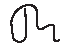
\includegraphics[height = 12px]{static/signature.pdf}
  \lv{name},
  \lv{neptun}
}

\renewcommand{\thesubsection}{\thesection.\alph{subsection}}

% Math related stuff goes here
\usepackage{amsmath}
\usepackage{amssymb}
\usepackage{fontspec}
\usepackage{unicode-math}

% Set font to my liking
\setmainfont{TeX Gyre Termes}
\setsansfont[Scale=MatchUppercase]{TeX Gyre Heros}
\setmathfont{Asana Math}

% Variable printing according to Hungarian standards
\usepackage{icomma}
\usepackage{siunitx}
\sisetup{
  per-mode = symbol,
  locale=DE
}

% Math custom commands
\newcommand\iu{\mathbf{j}}
\newcommand{\rvec}[1]{\mathbfit{#1}}
\newcommand{\uvec}[1]{\widehat{\mathbfit{#1}}}
\newcommand{\rmat}[1]{\mathbf{#1}}

% Operator like commands
\DeclareMathOperator\atann{atan2}

% Switching between SI modes
\newcommand{\sifigures}[1]{\sisetup{exponent-mode = fixed, round-mode=figures, round-precision=#1}}
\newcommand{\siplaces}[1]{\sisetup{exponent-mode = fixed, round-mode=places, round-precision=#1}}
\newcommand{\sisci}{\sisetup{exponent-mode = scientific}}

\usepackage{tikz}
\usepackage{pgfplots}
\pgfplotsset{compat=1.18, width=16cm, height=7.867cm}
\usepgfplotslibrary{fillbetween}
\pgfkeys{/pgf/number format/use comma}
\pgfkeys{/pgf/number format/1000 sep={\,}}
\pgfplotsset{%
  xmin=0,xmax=\lv{c}*1.05,
  every major tick/.style = {gray, semithick},
  axis x line=center,  axis y line=center,
  enlarge y limits=.05,
  axis line style={-to, thick},
  grid=both,
  grid style={line width=.1pt, draw=gray!20},
  major grid style={line width=.2pt,draw=gray!80},
  scaled y ticks=false,
}
\usetikzlibrary{
  calc,
  angles,
  quotes,
  backgrounds,
  patterns,
  arrows,
  arrows.meta,
  positioning,
  intersections,
  shapes.geometric,
}

\tikzset{
  dot/.style = {
      circle,
      fill=red!80!gray,
      minimum size=#1,
      draw=black,
      inner sep=0pt, outer sep=0pt,
      very thick,
    },
  dot/.default = 7pt,
  gdot/.style = {
      dot,
      fill=white
    },
  dim/.style = {
      latex-latex,
      draw=teal,
      ultra thick
    },
  joint/.style = {
      circle,
      draw=black,
      ultra thick,
      fill=cyan!20,
      minimum size=4mm,
    },
  square/.style = {
      regular polygon,
      regular polygon sides=4
    },
  rod/.style = {
      rectangle,
      draw=black,
      minimum height=6mm,
      minimum width=6mm,
      fill=yellow!10,
      ultra thick,
      midway,
      outer sep=0,
    },
}

% Other included packages go here
\usepackage{tabto}
\usepackage{multicol}
\usepackage{xcolor}
\usepackage{float}
\usepackage{array}
\usepackage{graphicx}
\newcolumntype{x}[1]{>{\centering\arraybackslash\hspace{0pt}}p{#1}}
\newcolumntype{X}[1]{>{$}x{#1}<{$}}


\begin{document}

\AddToShipoutPictureFG*{
  \setmainfont{Latin Modern Roman}
  \setmathfont{Latin Modern Math}
  \put(12cm,27.33cm){
    \makebox(7.5cm,1cm){
      \hfill \lv{name}
    }
  }
  \put(12cm,26.67cm){
    \makebox(7.5cm,1cm){
      \hfill \lv{neptun}
    }
  }
  \put(15.45cm,26cm){
    \makebox(7.5cm,1cm){
      \hfill 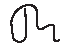
\includegraphics[height=5mm]{./static/signature.pdf} \hfill
    }
  }

  \put(9.5cm,25cm){
    \makebox(15mm,0){\lvec{code}{1}}
    \makebox(8.75mm,0){\lvec{code}{2}}
    \makebox(8.95mm,0){\lvec{code}{3}}
    \makebox(8.75mm,0){\lvec{code}{4}}
  }
}
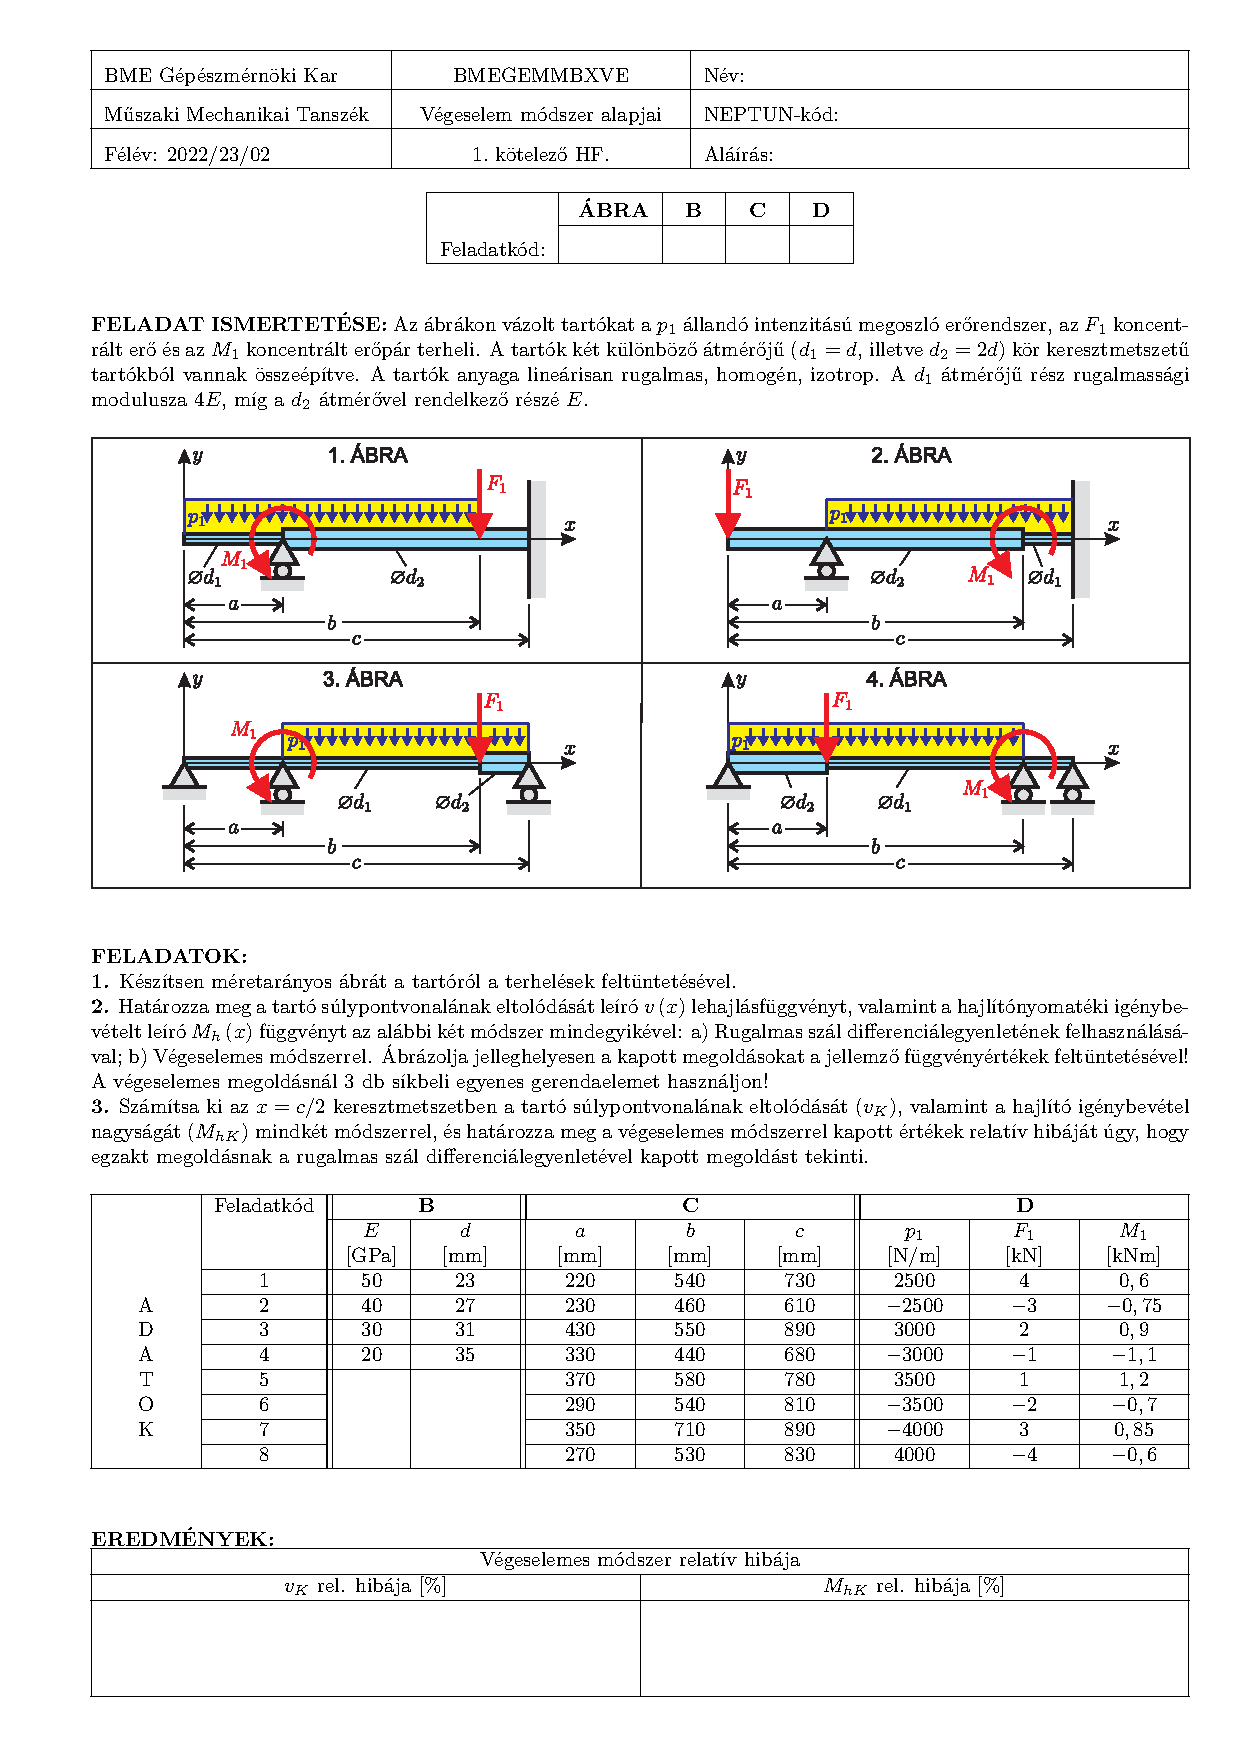
\includepdf[
  pages=-,
  scale=.95,
  pagecommand=\thispagestyle{fancy}
]{static/titlepage.pdf}
\setmainfont{TeX Gyre Termes}
\setmathfont{Asana Math}


\section{Méretarányos ábra} % (fold)
\label{sec:Méretarányos ábra}

A feladatkódom (\texttt{\lvec{code}{1}\lvec{code}{2}\lvec{code}{3}\lvec{code}{4}})
alapján a szerkezetet jellemző adatok:
\begin{multicols}{3}
  \begin{itemize}
    \item $a = \silv{a}{m}$,
    \item $b = \silv{b}{m}$,
    \item $c = \silv{c}{m}$,

    \item $p_1 = p_t = \silv{p_t}{N/m}$.
    \item $F_1 = F_t = \silv{F_t}{N}$.
    \item $M_1 = M_t = \silv{M_t}{Nm}[0]$,

    \item $\siplaces{0}\sisci{}E = \silv{E}{Pa}$,
    \item $d = \silv{d}{m}$.
  \end{itemize}
\end{multicols}

A megadott adatok alapján a szerkezetről készített méretarányos vázlat az
\ref{fig:construction}. ábrán látható. A lapon mért $\SI{1}{cm}$ távolság
a valóságban $\SI{10}{cm}$-nek felel meg.

\begin{figure}[H]
  \centering
  \includestandalone{construction}
  \caption{Méretarányos ábra a tartóról}
  \label{fig:construction}
\end{figure}

% section Méretarányos ábra (end)



\section{Lehajlás-, és hajlítónyomatéki igénybevétel függvények} % (fold)
\label{sec:Lehajlás- és hajlítónyomatéki igénybevétel függvények}

\begin{figure}[H]
  \centering
  \includestandalone{numbering}
  \vspace{-2mm}
  \caption{A csomópontok és elemek számozása}
  \label{fig:numbering}
\end{figure}

\vspace{-2mm}
A keresett függvényeket először szilárdságtani, majd pedig végeselemes
módszer segítségével fogjuk meghatározni. Számítsuk ki először azokat a
paramétereket, melyeket mindkét megoldás fel fogunk használni.

\bgroup
\begin{multicols}{2}
  A vékonyabb gerenda paraméterei:
  \begin{itemize}
    \item $d_1 = d = \silv{d_1}{m}$
          \sisci{} \siplaces{0}
    \item $E_1 = 4E = \silv{E_1}{Pa}$
          \siplaces{4}
    \item $A_1 = \dfrac{{d_1}^2 \pi}{4} = \silv{A_1}{m^2}$
          \siplaces{4}
    \item $I_1 = \dfrac{{d_1}^4 \pi}{64} = \silv{I_1}{m^4}$
  \end{itemize}
  A vastagabb gerenda paraméterei:
  \begin{itemize}
    \item $d_2 = 2d = \silv{d_2}{m}$
          \sisci{} \siplaces{0}
    \item $E_2 = E = \silv{E_2}{Pa}$
          \siplaces{4}
    \item $A_2 = \dfrac{{d_2}^2 \pi}{4} = \silv{A_2}{m^2}$
          \siplaces{4}
    \item $I_2 = \dfrac{{d_2}^4 \pi}{64} = \silv{I_2}{m^4}$
  \end{itemize}
\end{multicols}
\egroup

Az egyes elemekhez és csomópontokhoz hozzárendelt sorszámok a
\ref{fig:numbering}. ábra tartalmazza.

A csomópontok koordinátáit az \ref{table:U}. táblázat tartalmazza.
\begin{table}[H]
  \def\arraystretch{1.1}
  \centering
  \caption{A csomópontok koordinátái}
  \begin{tabular}{| c || X{1.5cm} | X{1.5cm} |}
    \hline
    Csp. & x \,[\text{m}] & y \,[\text{m}]
    \\ \hline \hline
    1    & \SI{0}{m}      & \SI{0}{m}
    \\ \hline
    2    & \silv{a}{m}    & \SI{0}{m}
    \\ \hline
    3    & \silv{b}{m}    & \SI{0}{m}
    \\ \hline
    4    & \silv{c}{m}    & \SI{0}{m}
    \\ \hline
  \end{tabular}
  \label{table:U}
\end{table}

Az egyes elemekhez tartozó csomópontokat, valamint további paramétereiket
a \ref{table:lok}. táblázat foglalja össze.
\begin{table}[H]
  \def\arraystretch{1.1}
  \centering
  \caption{Elem -- csomópont összerendelések}
  \begin{tabular}{| c || c | c || *{5}{>{$}c<{$}|}}
    \hline
    Elem & 1. csp & 2. csp & d                          & L         & A                          & E                          & I                          \\ \hline \hline
    1    & 1      & 2      & d_\dv{P.beams[1]['value']} & L_1 = a-0 & A_\dv{P.beams[1]['value']} & E_\dv{P.beams[1]['value']} & I_\dv{P.beams[1]['value']} \\ \hline
    2    & 2      & 3      & d_\dv{P.beams[2]['value']} & L_2 = b-a & A_\dv{P.beams[2]['value']} & E_\dv{P.beams[2]['value']} & I_\dv{P.beams[2]['value']} \\ \hline
    3    & 3      & 4      & d_\dv{P.beams[3]['value']} & L_3 = c-b & A_\dv{P.beams[3]['value']} & E_\dv{P.beams[3]['value']} & I_\dv{P.beams[3]['value']} \\ \hline
  \end{tabular}
  \label{table:lok}
\end{table}




\subsection{Megoldás differenciálegyenlettel} % (fold)
\label{ssec:Megoldás differenciálegyenlettel}

Írjuk fel az $y$ és $z$ irányú egyensúlyi egyenleteket:




% subsection Megoldás differenciálegyenlettel (end)


\subsection{Megoldás végeselem módszerrel} % (fold)
\label{ssec:Megoldás végeselem módszerrel}

A végeselem modellünkben jelenleg 4 csomópont van, ezért a rendszernek összesen
$4 \cdot 2 = 8$ szabadsági foka van. A rendszer csomóponti elmozdulásvektora
emiatt $8$ elemű:
\begin{equation}
  \rvec{U} = \left[ \begin{array}{*{8}{X{6mm}}}
      v_1 & \varphi_1 &
      v_2 & \varphi_2 &
      v_3 & \varphi_3 &
      v_4 & \varphi_4
    \end{array}
    \right]^\mathsf{T}\text{.}
  \label{eq:U-params}
\end{equation}

Az egyes elemekhez tartozó elmozdulásvektorok:
\begin{gather}
  \rvec{U}_1 = \left[ \begin{array}{*{4}{X{6mm}}}
      v_1 & \varphi_1 &
      v_2 & \varphi_2
    \end{array}
    \right]^\mathsf{T}
  \text,
  \\
  \rvec{U}_2 = \left[ \begin{array}{*{4}{X{6mm}}}
      v_2 & \varphi_2 &
      v_3 & \varphi_3
    \end{array}
    \right]^\mathsf{T}
  \text,
  \\
  \rvec{U}_3 = \left[ \begin{array}{*{4}{X{6mm}}}
      v_3 & \varphi_3 &
      v_4 & \varphi_4
    \end{array}
    \right]^\mathsf{T}
  \text.
\end{gather}

Határozzuk meg az egyes elemekhez tartozó merevségi mátrixokat. Egy ilyen mátrix
síkbeli gerendák esetén az alábbi alakot veszi fel:
\begin{equation}
  \rmat K_i
  = \frac{I_i E_i}{L_i}
  \begin{bmatrix}
    12    & 6 L_i     & -12    & 6 L_i     \\
    6 L_i & 4 {L_i}^2 & -6 L_i & 2 {L_i}^2 \\
    -12   & -6 L_i    & -2     & -6 L_i    \\
    6 L_i & 2 {L_i}^2 & -6 L_i & 4 {L_i}^2 \\
  \end{bmatrix}
  \text.
  \label{eq:Ke-param}
\end{equation}

Az elemi merevségi mátrixok numerikusan:
\bgroup
\siplaces{1}
\begin{align}
  \directlua{H.fullKei()}
\end{align}
\egroup

A globális merevségi mátrix meghatározásához írjuk fel az egyes elemekhez
tartozó szabadsági fokokat mátrixosan:
\begin{equation}
  \directlua{H.printDOFMatrix()}
  \label{eq:DOF}
\end{equation}

\subsubsection{A globális merevségi mátrix összeállítása}

A globális merevségi mátrix összeállításakor figyelnünk kell arra, hogy az adott
elem merevségi mátrixának megfelelő elemeit a hozzá tartozó szabadsági fokhoz
tartozó helyhez rendeljük hozzá. Ezt a \ref{fig:K}. ábra szemlélteti.
\begin{figure}[H]
  \centering
  \includestandalone{K-construction}
  \caption{A globális merevségi mátrix szemléletes felépítése}
  \label{fig:K}
\end{figure}

A globális merevségi mátrix tehát az alábbi alakot veszi fel:
\begin{equation}
  \siplaces{3}
  \rmat K = \begin{bmatrix}
    \directlua{H.printK(1e-6)}
  \end{bmatrix} \cdot 10^6 \, \mathrm{SI}
  \text.
  \label{eq:K}
\end{equation}

\subsubsection{A merevségi egyenlet}

A globális terhelésvektor a reakciók és a terhelések összege. Az állandó
intenzitású megoszló terhelést az elemek végén ébredő koncentrált erőkkel
és erőpárokkal helyettesítjük. A vektor a kényszerek ismeretében az alábbi
alakot veszi fel:
\begin{equation}
  \def\arraystretch{1.2}
  \rvec{F} =
  \directlua{H.printParametricF()}
  \label{eq:F-param}
\end{equation}

A rendszer merevségi egyenlete:
\begin{equation}
  \rmat K \rvec U = \rvec F
  \text.
  \label{eq:KUF}
\end{equation}

Fontos, hogy a merevségi egyenlet csak abban az esetben oldható meg mátrix
inverziós módszerrel, amennyiben $\rmat K$ mátrix reguláris. Mivel ez a
feltétel nem teljesül, ezért keressünk peremfeltételeket, melyek segítségével
olyan alakra redukáljuk az egyenletrendszert, hogy az invertálással megoldható
legyen. A szerkezet felépítése alapján tudjuk, hogy
%
% \begin{noindent}
\begin{luacode*}
  local connections = V.parametric.connections
  local len  = #connections

  for i=1,len do
    local type = connections[i].dof
    local loc = connections[i].l
    

    if i == 1 then
      tex.sprint "az "
    else 
      tex.sprint "a "
    end
    tex.sprint([[($]] .. loc:upper() .. [[$) pontban lévő]])

    if type == 1 then
      tex.sprint [[ görgős támasz]]
    elseif type == 2 then
      tex.sprint [[ csuklós támasz]]
    elseif type == 3 then
      tex.sprint [[ befogás]]
    end

    if i == len - 1 then
      tex.sprint [[, valamint  ]]
    elseif i == len then
      tex.sprint [[ miatt ]]
    else
      tex.sprint [[, ]]
    end
  end
\end{luacode*}
% \end{noindent}
az alábbi peremfeltételeket kapjuk:
\begin{equation}
	% \begin{noindent}
  \begin{luacode*}
    local notFree = V.parametric.notFree

    for k=1,3 do
      local i = notFree[k]
      local j = math.floor((i+1)/2)

      if i%2 == 1 then
        tex.sprint("v_" .. j .. "=0")
      else
        tex.sprint("\\varphi_" .. j .. "=0")
      end

      if k==3 then
        tex.sprint [[ \text. ]]
      else
        tex.sprint [[ \text,\quad ]]
      end
    end
  \end{luacode*}
  % \end{noindent}
\end{equation}
Ezen adatok ismeretében már fel tudjuk írni a kondenzált merevségi egyenletet,
melyet úgy kapunk meg, hogy a  gátolt szabadsági fokokhoz tartozó sorokat és
oszlopokat töröljük az eredeti, globális merevségi egyenletből:
\begin{equation}
	\sifigures{3} \sisci{}
	\underbrace{\begin{bmatrix}
			\directlua{H.printKkond()}
		\end{bmatrix}}_{\widehat{\rmat K}}
	% \begin{noindent}
  \begin{luacode*}
    tex.sprint [[\underbrace{\begin{bmatrix}]]
    local free = V.parametric.free

    for k=1,5 do
      local i = free[k]
      local j = math.floor((i+1)/2)

      if i%2 == 1 then
        tex.sprint("v_" .. j .. "\\\\")
      else
        tex.sprint("\\varphi_" .. j .. "\\\\")
      end
    end
    tex.sprint [[\end{bmatrix}}_{\widehat{\rvec U}}]]
  \end{luacode*}
  % \end{noindent}
	=
	\siplaces{2} \sifix{}
	\underbrace{\begin{bmatrix}
			\directlua{H.printFkond()}
		\end{bmatrix}}_{\widehat{\rvec F}}
	\text.
	\label{eq:cond}
\end{equation}


%
Mivel $\widehat{\rmat K}$ mátrix reguláris, ezért az egyenletrendszer
mátrix-invertálással megoldható, vagyis:
\begin{equation}
  \sifigures{3} \sisci{}
  \widehat{\rvec U} =
  \underbrace{\begin{bmatrix}
      \directlua{H.printKinv()}
    \end{bmatrix}}_{\widehat{\rmat K}^{-1}}
  \siplaces{2} \sifix{}
  \underbrace{\begin{bmatrix}
      \directlua{H.printFkond()}
    \end{bmatrix}}_{\widehat{\rvec F}}
  .
  \label{eq:inverted}
\end{equation}

Az egyenlet megoldása numerikusan:
\begin{equation}
  \sifigures{4} \sisci{}
  \widehat{\rvec U} = \begin{bmatrix}
    \directlua{H.printUkond(1)}
  \end{bmatrix} \, \mathrm{SI}
  =
  \siplaces{4} \sifix{}
  \begin{bmatrix}
    \directlua{H.printUkondDegMM()}
  \end{bmatrix}
  \text.
  \label{eq:numericCond}
\end{equation}

A globális elmozdulásvektorba visszahelyettesítve:
\begin{equation}
  \sifigures{3} \sisci\
  {\rvec U} = \begin{bmatrix}
    \directlua{H.printUcalc()}
  \end{bmatrix} \, \mathrm{SI}
  =
  \siplaces{4} \sifix{}
  \begin{bmatrix}
    \directlua{H.printUcalcDegMM()}
  \end{bmatrix}
  \text.
\end{equation}

Ha a merevségi egyenletbe visszahelyettesítjük a már ismert elmozdulási vektort,
akkor megkaphatjuk a terhelési vektort numerikusan:
\begin{equation}
  \siplaces{3}
  \rvec F = \rmat K \rvec U =
  \begin{bmatrix}
    \directlua{H.printFcalc()}
  \end{bmatrix}
  \, \mathrm{SI}
  =
  \underbrace{\begin{bmatrix}
      \directlua{H.printF()}
    \end{bmatrix}}_\text{terhelés}
  \, \mathrm{SI}
  +
  \underbrace{\begin{bmatrix}
      \directlua{H.printFreacc()}
    \end{bmatrix}}_\text{reakció}
  \, \mathrm{SI}
  \text.
  \label{eq:Fcalc}
\end{equation}

\subsubsection{Keresett függvények meghatározása}

A lehajlás- és szögelfordulás függvények meghatározásához elemeken belüli 
interpolációt kell alkalmaznunk. A formafüggvények alakja a globális 
koordináta-rendszerben:
\begin{equation}
  \renewcommand\a{\left(\sfrac{x}{L_i}\right)}
  \rvec N(x) =
  \begin{bmatrix}
    1 - 3\a^2 + 2\a  \\[2mm]
    x - 2x\a + x\a^2 \\[2mm]
    3\a^2 - 2\a^3    \\[2mm]
    -x\a + x\a^2
  \end{bmatrix}
  \text.
  \label{eq:N-param}
\end{equation}

Tetszőleges elem lehajlásfüggvénye előállítható az alábbi módon:
\begin{equation}
  v_i(x) = \rvec N(x)^{\mathsf T} \rvec U_i
  \text.
  \label{eq:v-param}
\end{equation}

Az elmozdulások ismeretében a függvények numerikusan:
\bgroup
\siplaces{6}
% \begin{noindent}
\begin{luacode*}
  tex.sprint [[\begin{alignat}{9}]]
  for i=1,3 do
    tex.sprint("v_" .. i .. "(x)&=\\,")

    local vMat = V.vMat

    for k=3,0,-1 do
      local value = vMat[i][k]

      if math.abs(value) >= 1e-16 then
        if value > 0 and k ~= 3 then
          tex.sprint "&+&"
        else
          tex.sprint "&-&"
        end
        H.printSIDirect {value=math.abs(value), unit="", dec=6}

        tex.sprint "&\\,"
        if k == 0 then
          tex.sprint ""
        elseif  k== 1 then 
          tex.sprint "x"
        else
          tex.sprint("x^" .. k)
        end
        tex.sprint("\\,")
      else
        tex.sprint("&&&")
      end
    end

    tex.sprint("&[\\mathrm m] \\text{,\\quad ha} \\quad x \\in (" .. ({0, 'a', 'b'})[i] .. ";" .. ({'a', 'b', 'c'})[i] .. ")")

    if i ~= 3 then
      tex.sprint "\\text,\\\\"
    else
      tex.sprint "\\text."
    end
  end
  tex.sprint [[\end{alignat}]]
\end{luacode*}
% \end{noindent}
\egroup


A szögelfordulás függvényeket megkapjuk, ha deriváljuk a lehajlásfüggvényeket:
\begin{equation}
  \varphi_i(x) = v_i'(x)
  \text.
  \label{eq:phi-param}
\end{equation}

A függvények numerikusan:
\bgroup
\siplaces{6}
% \begin{noindent}
\begin{luacode*}
  tex.sprint [[\begin{alignat}{9}]]
  for i=1,3 do
    tex.sprint("\\varphi_" .. i .. "(x)&=\\,")

    local phiMat = V.phiMat

    for k=2,0,-1 do
      local value = phiMat[i][k]

      if math.abs(value) >= 1e-16 then
        if value > 0 and k ~= 3 then
          tex.sprint "&+&"
        else
          tex.sprint "&-&"
        end
        H.printSIDirect {value=math.abs(value), unit="", dec=6}

        tex.sprint "&\\,"
        if k == 0 then
          tex.sprint ""
        elseif  k == 1 then 
          tex.sprint "x"
        else
          tex.sprint("x^" .. k)
        end
        tex.sprint("\\,")
      else
        tex.sprint("&&&")
      end
    end

    tex.sprint("[&\\mathrm{rad}] \\text{,\\quad ha} \\quad x \\in (" .. ({0, 'a', 'b'})[i] .. ";" .. ({'a', 'b', 'c'})[i] .. ")")

    if i ~= 3 then
      tex.sprint "\\text,\\\\"
    else
      tex.sprint "\\text."
    end
  end
  tex.sprint [[\end{alignat}]]
\end{luacode*}
% \end{noindent}
\egroup


A rugalmas szál differenciálegyenlete alapján a hajlítónyomatéki függvények
és lehajlások közötti kapcsolat:
\begin{equation}
  M_{h,i}(x) = -IE \cdot v_i''(x)
  \text.
  \label{eq:Mh-param}
\end{equation}

A függvények numerikusan:
\bgroup
\sifigures{6}
% \begin{noindent}
\begin{luacode*}
  tex.sprint [[\begin{alignat}{9}]]
  for i=1,3 do
    tex.sprint("M_{h" .. i .. "}(x)&=\\,")

    local MhMat = V.MhMat

    for k=1,0,-1 do
      local value = MhMat[i][k]

      if math.abs(value) >= 1e-16 then
        if value > 0 and k ~= 3 then
          tex.sprint "&+&"
        else
          tex.sprint "&-&"
        end
        H.printSIDirect {value=math.abs(value), unit="", dec=6}

        tex.sprint "&\\,"
        if k == 0 then
          tex.sprint ""
        elseif  k == 1 then 
          tex.sprint "x"
        end
        tex.sprint("\\,")
      else
        tex.sprint("&&&")
      end
    end

    tex.sprint("[&\\mathrm{Nm}] \\text{,\\quad ha} \\quad x \\in (" .. ({0, 'a', 'b'})[i] .. ";" .. ({'a', 'b', 'c'})[i] .. ")")

    if i ~= 3 then
      tex.sprint "\\text,\\\\"
    else
      tex.sprint "\\text."
    end
  end
  tex.sprint [[\end{alignat}]]
\end{luacode*}
% \end{noindent}
\egroup

% A végeselem módszerrel kapott függvények értékei a nevezetes pontokban:
% \begin{noindent}
\begin{table}[H]
\centering
\caption{A végeselem módszerrel kapott függvényértékek a nevezetes pontokban}
\sifix{}
\def\arraystretch{1.25}
\begin{luacode*}
  tex.sprint[[\begin{tabular}{c|c|c|c|c|}]]
  tex.sprint[[& $x = 0$ & $x = a$ & $x = b$ & $x = c$ \\\hline]]

  tex.sprint [[$v(x)$]]

  for i=1,4 do
    local num = V.bNum[1][i]
    tex.sprint [[&]]
    if math.abs(num) < 1e-10 then
      tex.sprint [[$0\,\mathrm{m}$]]
    else
      H.printSIDirect { value = num, unit="m", dec=6 }
    end
  end

  tex.sprint [[\\]]

  tex.sprint [[$\varphi(x)$]]

  for i=1,4 do
    local num = V.bNum[2][i]
    tex.sprint [[&]]
    if math.abs(num) < 1e-10 then
      tex.sprint [[$0\,\mathrm{rad}$]]
    else
      H.printSIDirect { value = num, unit="rad", dec=6 }
    end
  end

  tex.sprint [[\\]]

  tex.sprint [[$M_h(x)$ & $-$]]

  for i=2,4 do
    local num = V.bNum[3][i]
    tex.sprint [[&]]
    if math.abs(num) < 1e-10 then
      tex.sprint [[$0\,\mathrm{Nm}$]]
    else
      H.printSIDirect { value = num, unit="Nm", dec=3 }
    end
  end

  tex.sprint [[\\]]

  tex.sprint [[$M_h(x)$]]

  for i=1,3 do
    local num = V.bNum[4][i]
    tex.sprint [[&]]
    if math.abs(num) < 1e-10 then
      tex.sprint [[$0\,\mathrm{Nm}$]]
    else
      H.printSIDirect { value = num, unit="Nm", dec=3 }
    end
  end

  tex.sprint [[&$-$\\\hline]]

  tex.sprint[[\end{tabular}]]
\end{luacode*}
\end{table}
% \end{noindent}



% subsection Megoldás végeselem módszerrel (end)

\begin{equation}
  \begin{array}{c}
    \directlua{H.xd()}
  \end{array}
  \label{eq:xd}
\end{equation}

\clearpage
\subsection{Megoldásfüggvények ábrázolása} % (fold)
\label{sub:Megoldásfüggvények ábrázolása}

\begin{figure}[H]
  \flushright
  \includestandalone{plot-v}
  \hspace{5mm}\vspace{-3mm}
  \caption{VEM és \textcolor{cyan!40!black}{ana}\textcolor{yellow!40!black}{liti}\textcolor{red!40!black}{kus} módszerekkel kapott $v(x)$ lehajlásfüggvény}
  \label{fig:plot-v}
\end{figure}

\begin{figure}[H]
  \flushright
  \includestandalone{plot-phi}
  \hspace{5mm}\vspace{-3mm}
  \caption{$\varphi(x)$}
  \label{fig:plot-phi}
\end{figure}

\begin{figure}[H]
  \flushright
  \includestandalone{plot-Mh}
  \hspace{5mm}\vspace{-3mm}
  \caption{$M_h(x)$}
  \label{fig:plot-Mh}
\end{figure}


% subsection Megoldásfüggvények ábrázolás (end)


% section Lehajlás-, és hajlítónyomatéki igénybevétel függvények (end)

\end{document}
